\chapter{多特征多分类器组合}

\section{基本原理}

本文选择了三类特征,对这三类特征分别用不同的分类算法进行分类,效果都不是很好,针对单个分类器不能完全表达浮游动物分类信息的情况,我们提出了一种基于多特征多分类器组合的浮游动物图像分类算法,框架如图~\ref{fig: framework}所示。首先,对浮游动物图像进行预处理以去除噪声。然后,对预处理后的图像提取三种不同类型的特征作为低层次特征。再将这些低层次特征输入到相应的机器学习算法,得到训练集中的每一幅图像在每一特征下被分到各个浮游生物图像类别中的概率,这个概率就作为中层次特征。最后,将三种类型特征对应的三种中层次特征串联起来并用支持向量机方法进行训练,得到最终的分类器。

\begin{figure}[!ht]
\centering
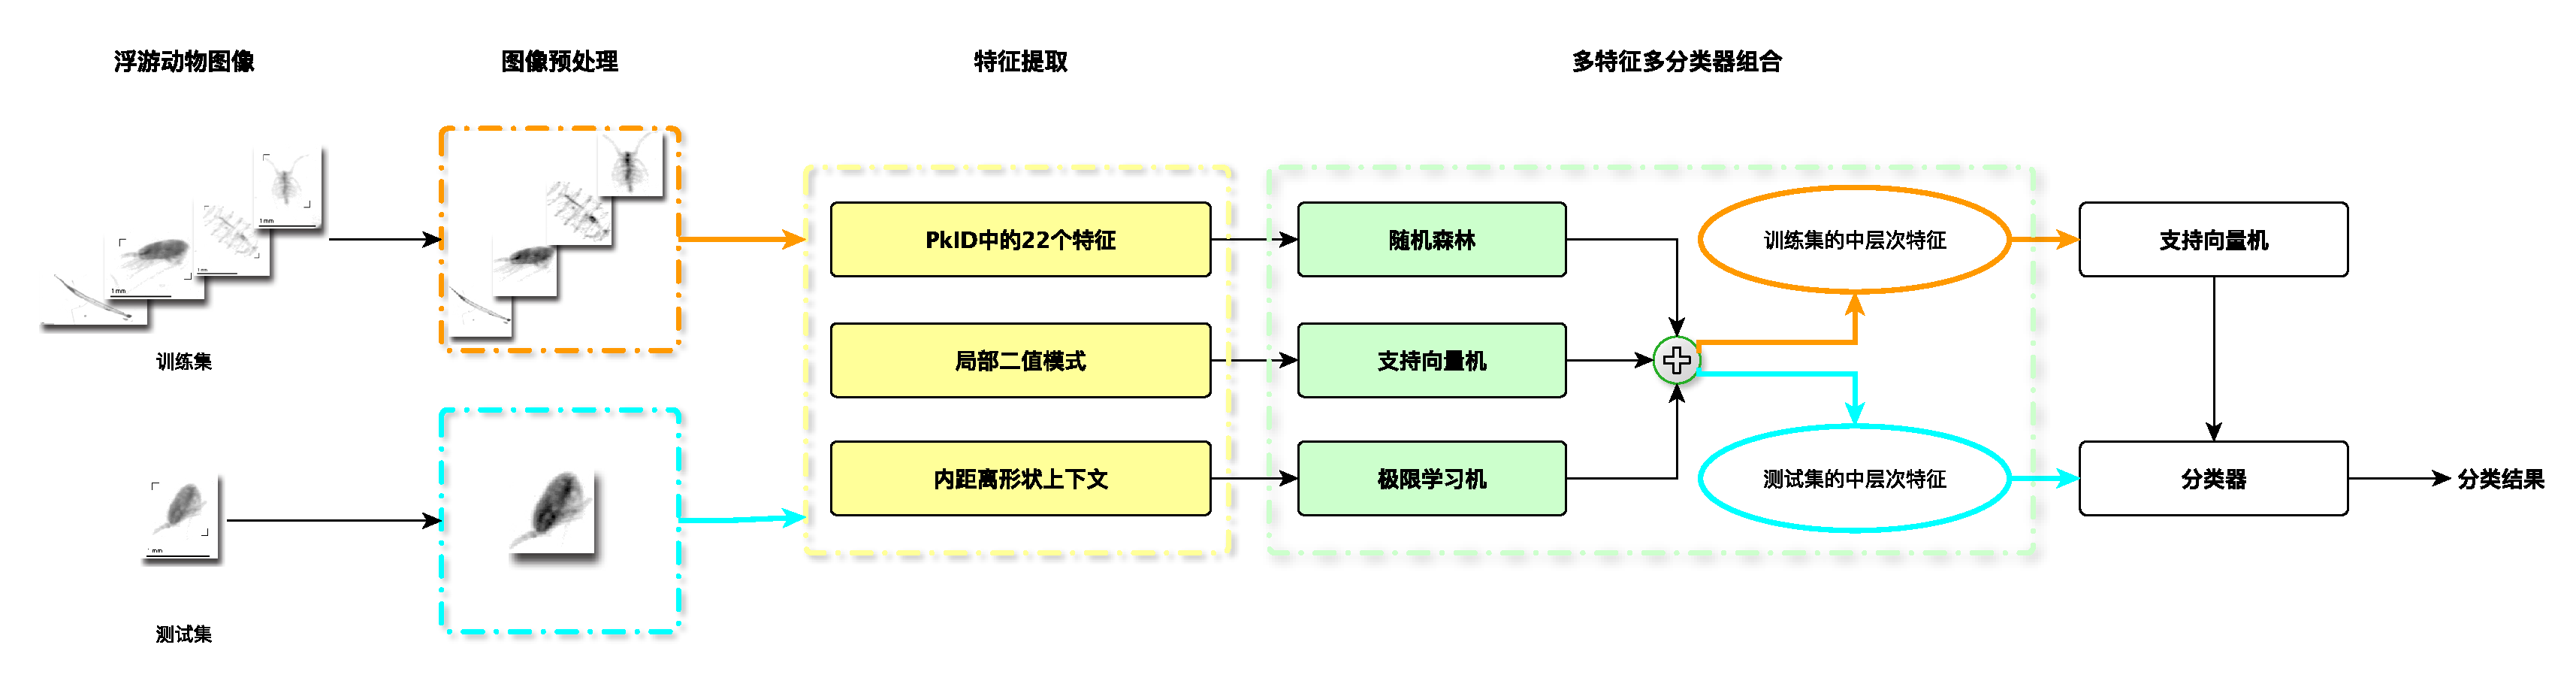
\includegraphics[width=1.0\linewidth]{framework.png}
\caption{基于多特征多分类器组合的浮游动物图像分类算法框架}
\label{fig: framework}
\end{figure}

在实验中,我们往往希望提取尽可能多的特征,以增强对图像或物体类别的描述,使分类效果更理想。但实际上特征数目与分类有效性之间并不是线性关系,很多特征本身可能只包含了少量有用信息,亦或者是带有一些冗余信息,这些都会对分类效果产生不好的影响。在第~\ref{3.1}和~\ref{2.3.3}节中,我们整理和总结了各种不同的特征,通过实验与分析,本文最终选取出的三类特征分别是PkID中的特征、局部二值模式和内距离形状上下文。

选取出特征后,我们采用多个分类器组合的技术对提取的不同类型的特征作不同的处理,每一类型的特征都用相应的适合该类型特征的分类算法来进行训练。如果训练集中有$M$幅图像,$n$个类别,我们提取了$m$种不同类型的特征,每一种类型的特征对应一种相应的分类算法,那么经过每一个分类算法除了能得到一个分类器外,还能得到训练集中的每一幅图像被分为每个类别的概率,对于整个数据集就会得到一个$M \times n$的矩阵,因为有$m$种不同类型的特征,所以最终会得到一个$M \times (n * m)$的矩阵。将这个矩阵作为对训练集图像提取的中层次特征,选取相应的分类算法进行训练,得到最终的分类器。

\section{图像预处理}

由于成像过程中受到的各种各样的干扰,我们所收集到的浮游图像不可避免地会带有一些噪声信号,这些噪声的引入,会直接导致图像的不清晰,造成识别准确率的下降。图~\ref{fig: origin_preprocess}(a)显示的是一幅原始的浮游动物图像,可以看到除了浮游动物目标外,周围还混杂了一些悬浮物、污点等噪声信息,对图像进行预处理的目的就是去除这些噪声信息,而保留和增强图像中对分类有用的信息。本文所采取的预处理方法是先对图像进行二值化,然后去除面积小于一定值的连通区域,图~\ref{fig: origin_preprocess}(b)显示的是经过预处理后的图像,除浮游动物外的一些污点噪声已经被去除掉了。

\begin{figure}[t]
  \centering%
  \begin{subfigure}{0.3\linewidth}
    \includegraphics[height=4cm]{origin.png}
    \caption{}
  \end{subfigure}
  \hspace{4em}%
  \begin{subfigure}{0.3\linewidth}
    \includegraphics[height=4cm]{preprocess.png}
    \caption{}
  \end{subfigure}
  \caption{预处理前和预处理后的图像对比}
  \label{fig: origin_preprocess}
\end{figure}

\section{实验对比与分析}

在本文中,我们将所提出的基于多特征多分类器组合的浮游动物图像分类方法与ZooScan系统进行了对比,选用的数据集是~\ref{2.1}节中介绍的13类浮游动物图像集,评价方法采用的是$K$折交叉验证。

PkID软件中,有7种机器学习算法供选用,将所提取出的67个特征都用上,并且机器学习算法定为随机森林时,分类准确率最高,约为75\%,见表~\ref{PkID-RF}。

\begin{table}
\centering
\caption{PkID软件中随机森林分类器分类结果}
\begin{tabular}{c}
\includegraphics[width=1.0\linewidth]{PkID-RF.pdf}
\end{tabular}
\label{PkID-RF}
\end{table}

将我们的算法中得到的三个分类器特征(中层次特征)串联起来,输入到支持向量机分类算法中,得到最终的分类器。这里我们仍然对其中的内距离形状上下文的参数选取进行了一些实验。当内距离形状上下文特征中模板数目设为39时,得到的分类器对测试集的分类结果评价如表~\ref{20+IDSC39+LBP-Features-MATLAB}所示,其分类准确率为77.1\%。当内距离形状上下文特征中模板数目设为65时,得到的分类器对测试集的分类结果评价如表~\ref{20+IDSC65+LBP-Features-MATLAB}所示,其分类准确率为77.7\%。而当内距离形状上下文特征中模板数目设为104时,得到的分类器对测试集的分类结果评价如表~\ref{20+IDSC104+LBP-Features-MATLAB}所示,其分类准确率并没有变化,仍然为77.7\%。所以最终我们一般对内距离形状上下文特征中的模板数目设为65,这样既能在一定程度上提高分类准确率,又不会使运行速度变得过慢。

\begin{table}
\centering
\caption{多特征多分类器组合(内距离形状上下文特征采用39张图像作为模板)}
\begin{tabular}{c}
\includegraphics[width=1.0\linewidth]{20+IDSC39+LBP-Features-MATLAB.pdf}
\end{tabular}
\label{20+IDSC39+LBP-Features-MATLAB}
\end{table}

\begin{table}
\centering
\caption{多特征多分类器组合(内距离形状上下文特征采用65张图像作为模板)}
\begin{tabular}{c}
\includegraphics[width=1.0\linewidth]{20+IDSC65+LBP-Features-MATLAB.pdf}
\end{tabular}
\label{20+IDSC65+LBP-Features-MATLAB}
\end{table}

\begin{table}
\centering
\caption{多特征多分类器组合(内距离形状上下文特征采用104张图像作为模板)}
\begin{tabular}{c}
\includegraphics[width=1.0\linewidth]{20+IDSC104+LBP-Features-MATLAB.pdf}
\end{tabular}
\label{20+IDSC104+LBP-Features-MATLAB}
\end{table}

对比表~\ref{PkID-RF}和表~\ref{20+IDSC65+LBP-Features-MATLAB}可以看到,本文中所提出的基于多特征多分类器组合的浮游动物图像分类算法与ZooScan系统中的识别软件相比,在识别准确率上有了明显的提高。并且我们的方法在使用的特征数量上有所降低,只采用了24个特征。这24个特征又可以分为三类,对这三类特征分别利用不同的分类算法进行训练得到的单个分类器的分类效果比组合这三个分类器的效果要差,这是因为组合分类器正确利用了单个分类器提供的信息,从不同的角度反映了图像的特性,最终的结果表明本文提出的多特征多分类器组合的方法是有效的。
